
\chapter{Questionário de Avaliação do Protótipo}

\begin{figure}[H]
	\begin{Center}
		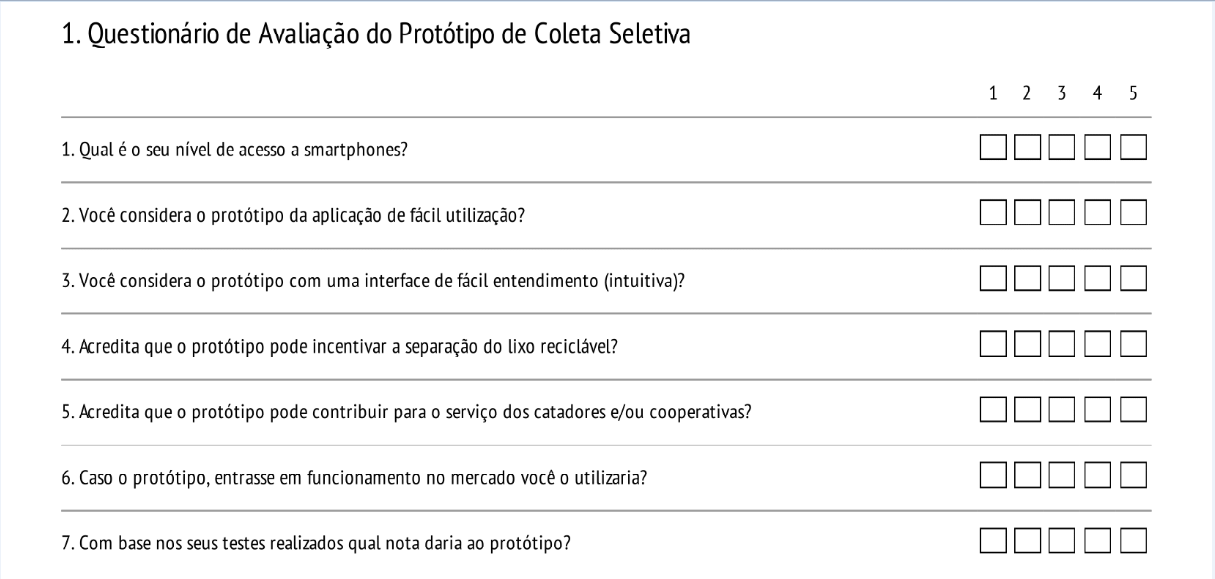
\includegraphics[width=6.00in]{media/questionariopaint.png}
		\label{fig:questionario}
	\end{Center}
\end{figure}

\chapter{Códigos fonte comentados}

\section{Salvar usuário catador no banco de dados}

O \autoref{cod:cadbanc} é responsável por salvar o usuário catador no \textit{firebase realtime database}. A linha 3 do \autoref{cod:cadbanc}, consiste na criação do nó (\textit{child}) denominado “Catadores”, onde cada catador possui um identificador (\textit{id}), onde seus dados são salvos (\textit{setValue}).

\begin{codigo}[H]
\begin{lstlisting}[language=Java]
public void salvar(){
    DatabaseReference databaseReference = ConfiguracaoFirebase.getFirebase();
    databaseReference.child("Catadores").child(getId()).setValue(this);
}
\end{lstlisting}
\caption{Salvar usuário catador no banco de dados}
\label{cod:cadbanc}
\end{codigo}


\section{Salvar usuário separador no banco de dados}

\begin{codigo}[H]
	\begin{lstlisting}[language=Java]
public void salvar(){
    DatabaseReference databaseReference = ConfiguracaoFirebase.getFirebase();
    databaseReference.child("Separadores").child(getId()).setValue(this);
}
   	\end{lstlisting}
   	\caption{Salvar usuário separador no banco de dados}
   	\label{cod:cadsep}
\end{codigo}

O \autoref{cod:cadsep} é responsável por salvar o usuário separador no \textit{firebase realtime database}. A linha 3 do \autoref{cod:cadbanc}, consiste na criação do nó (\textit{child}) denominado “Separadores”, onde cada separador possui um identificador (\textit{id}), onde seus dados são salvos (\textit{setValue}).


\section{Cadastrar usuário catador}

\begin{codigo}[H]
	\begin{lstlisting}[language=Java]
private void cadastrarCatador(){
    firebaseAuth = ConfiguracaoFirebase.getFirebaseAuth();
    firebaseAuth.createUserWithEmailAndPassword(
            catador.getEmail(),
            catador.getSenha()
    ).addOnCompleteListener(CadastroCatador.this, new OnCompleteListener<AuthResult>() {
        @Override
        public void onComplete(@NonNull Task<AuthResult> task) {
            if(task.isSuccessful()){
                Toast.makeText(CadastroCatador.this,"Sucesso ao cadastrar catador",Toast.LENGTH_LONG).show();
                FirebaseUser firebaseUser = task.getResult().getUser();
                catador.setId(firebaseUser.getUid());
                catador.salvar();
                startActivity(new Intent(CadastroCatador.this, Login.class));
       	\end{lstlisting}
       	\caption{Cadastrar usuário catador na aplicação}
       	\label{cod:cat}
\end{codigo}

O \autoref{cod:cat} consiste no cadastro do usuário catador. A função \textit{createUserWithEmailAndPassword}, que se encontra na linha 3, é responsável pela criação da autenticação dos usuário através do \textit{e-mail} e a senha. Em caso de sucesso, o sistema irá exibir a seguinte mensagem “Sucesso ao cadastrar catador” e o usuário será redirecionado para a tela de \textit{login}.

\section{Cadastrar usuário separador}

\begin{codigo}[H]
	\begin{lstlisting}[language=Java]
private void cadastrarSeparador(){
    firebaseAuth = ConfiguracaoFirebase.getFirebaseAuth();
    firebaseAuth.createUserWithEmailAndPassword(
            separador.getEmail(),
            separador.getSenha()
    ).addOnCompleteListener(CadastroSeparador.this, new OnCompleteListener<AuthResult>() {
        @Override
        public void onComplete(@NonNull Task<AuthResult> task) {
            if(task.isSuccessful()){
                Toast.makeText(CadastroSeparador.this,"Sucesso ao cadastrar separador",Toast.LENGTH_LONG).show();
                FirebaseUser firebaseUser = task.getResult().getUser();
                separador.setId(firebaseUser.getUid());
                separador.salvar();
                startActivity(new Intent(CadastroSeparador.this, Login.class));
       	\end{lstlisting}
       	\caption{Cadastrar usuário separador}
       	\label{cod:sep}
\end{codigo}

O \autoref{cod:sep} consiste no cadastro do usuário separador. A função \textit{createUserWithEmailAndPassword}, que se encontra na linha 3, é responsável pela criação da autenticação do usuário através do \textit{e-mail} e a senha. Em caso de sucesso, o sistema irá exibir a seguinte mensagem “Sucesso ao cadastrar separador” e o usuário será redirecionado para a tela de \textit{login}.

\section{Redefinir a senha}

\begin{codigo}[H]
	\begin{lstlisting}[language=Java]
	private void redefinirsenha(){
        firebaseAuth = FirebaseAuth.getInstance();
        firebaseAuth.sendPasswordResetEmail(recuperar.getEmail())
                .addOnCompleteListener(new OnCompleteListener<Void>() {
                    @Override
                    public void onComplete(@NonNull Task<Void> task) {
                        if(task.isSuccessful()) {
                            Toast.makeText(RecuperarSenha.this, "E-mail enviado.", Toast.LENGTH_LONG).show();
                            startActivity(new Intent(RecuperarSenha.this, Login.class));
                        }else{
                            Toast.makeText(RecuperarSenha.this,"E-mail nao cadastrado.",Toast.LENGTH_LONG).show();
                        }
                    }
                });
    }
    \caption{Redefinir a senha}
    \label{cod:senha}
 	\end{lstlisting}
\end{codigo}

O \autoref{cod:senha} consiste na redefinição da senha do usuário. A linha 3 verifica se o \textit{e-mail} informado pelo usuário está cadastrado no \textit{firebase auth}. Em caso de sucesso, o sistema irá enviar um \textit{e-mail} para a redefinição da senha e o usuário será redirecionado para a tela de \textit{login}. Caso contrário o sistema irá exibir a seguinte mensagem “\textit{E-mail} não cadastrado”.

\section{Deslogar usuário}
\begin{codigo}[H]
	\begin{lstlisting}[language=Java]
private void deslogarUsuario() {
        firebaseAuth.signOut();
        Toast.makeText(MapsActivity.this, "Usuario deslogado!", Toast.LENGTH_LONG).show();
        Intent intent = new Intent(MapsActivity.this, Login.class);
        startActivity(intent);
        finish();
    \end{lstlisting}
    \caption{Deslogar usuário}
    \label{cod:des}
\end{codigo}

O \autoref{cod:des} consiste no \textit{logout} do usuário. A função \textit{signOut} que encontra na linha 2 é responsável por desconectar o usuário da aplicação. A linha 3 tem a função de exibir para o usuário a seguinte mensagem "Usuario deslogado". A linha 4 tem o papel de redirecionar o usuário para a tela de \textit{login}.

\section{Validar separador}

\begin{codigo}[H]
	\begin{lstlisting}[language=Java]
private void validarSeparador() {
    firebaseAuth2 = ConfiguracaoFirebase.getFirebaseAuth();
    firebaseAuth2.signInWithEmailAndPassword(
        separador.getEmail(),
        separador.getSenha()
    ).addOnCompleteListener(new OnCompleteListener<AuthResult>() {
        @Override
        public void onComplete(@NonNull Task<AuthResult> task) {
            if (task.isSuccessful()) {
                FirebaseUser currentUser = FirebaseAuth.getInstance().getCurrentUser();
                assert currentUser != null;
                String id = currentUser.getUid();
                DatabaseReference j = FirebaseDatabase.getInstance().getReference().child("Separadores").child(id);
                j.addValueEventListener(new ValueEventListener() {
                    @Override
                    public void onDataChange(@NonNull DataSnapshot dataSnapshot)
                    {
                        String userType = (String) dataSnapshot.child("userType").getValue();
                        if (userType != null && userType.equals("Separadores")) {
                            Toast.makeText(Login.this, "Login efetuado com sucesso!", Toast.LENGTH_SHORT).show();
                            Intent intentResident = new Intent(Login.this, Materiais.class);
                            startActivity(intentResident);
                            finish();
                        }
                }
    	\end{lstlisting}
    	\caption{Validar separador}
    	\label{cod:valsep}
\end{codigo}

O \autoref{cod:valsep} consiste na validação do usuário separador. A verificação do tipo de usuário separador é realizada através da referência do nó "Separador", do identificador e do tipo de usuário.


\section{Validar catador}

\begin{codigo}[H]
	\begin{lstlisting}[language=Java]
private void validarCatador() {
    firebaseAuth2 = ConfiguracaoFirebase.getFirebaseAuth();
    firebaseAuth2.signInWithEmailAndPassword(
        catador.getEmail(),
        catador.getSenha()
    ).addOnCompleteListener(new OnCompleteListener<AuthResult>() {
        @Override
        public void onComplete(@NonNull Task<AuthResult> task) {
            if (task.isSuccessful()) {
                FirebaseUser currentUser = FirebaseAuth.getInstance().getCurrentUser();
                assert currentUser != null;
                String id = currentUser.getUid();
                DatabaseReference j = FirebaseDatabase.getInstance().getReference().child("Catadores").child(id);
                j.addValueEventListener(new ValueEventListener() {
                    @Override
                    public void onDataChange(@NonNull DataSnapshot dataSnapshot)
                    {
                        String userType = (String) dataSnapshot.child("userType").getValue();
                        if (userType != null && userType.equals("Catador")) {
                            Toast.makeText(Login.this, "Login efetuado com sucesso!", Toast.LENGTH_SHORT).show();
                            Intent intentResident = new Intent(Login.this, Servicos.class);
                            startActivity(intentResident);
                            finish();
                        }
                }
    	\end{lstlisting}
    	\caption{Validar catador}
    	\label{cod:valcat}
\end{codigo}

O \autoref{cod:valcat} consiste na validação do usuário catador. A verificação do tipo de usuário catador é realizada através da referência do nó "Catadores", do identificador e do tipo de usuário.

\section{Traçar rota}

\begin{codigo}[H]
	\begin{lstlisting}[language=Java]
	private void parseJSon(String data) throws JSONException {
        if (data == null)
            return;
        List<Route> routes = new ArrayList<Route>();
        JSONObject jsonData = new JSONObject(data);
        JSONArray jsonRoutes = jsonData.getJSONArray("routes");
        for (int i = 0; i < jsonRoutes.length(); i++) {
            JSONObject jsonRoute = jsonRoutes.getJSONObject(i);
            Route route = new Route();
            JSONObject overview_polylineJson = jsonRoute.getJSONObject("overview_polyline");
            JSONArray jsonLegs = jsonRoute.getJSONArray("legs");
            JSONObject jsonLeg = jsonLegs.getJSONObject(0);
            JSONObject jsonDistance = jsonLeg.getJSONObject("distance");
            JSONObject jsonDuration = jsonLeg.getJSONObject("duration");
            JSONObject jsonEndLocation = jsonLeg.getJSONObject("end_location");
            JSONObject jsonStartLocation = jsonLeg.getJSONObject("start_location");
            route.distance = new Distance(jsonDistance.getString("text"), jsonDistance.getInt("value"));
            route.duration = new Duration(jsonDuration.getString("text"), jsonDuration.getInt("value"));
            route.endAddress = jsonLeg.getString("end_address");
            route.startAddress = jsonLeg.getString("start_address");
            route.startLocation = new LatLng(jsonStartLocation.getDouble("lat"), jsonStartLocation.getDouble("lng"));
            route.endLocation = new LatLng(jsonEndLocation.getDouble("lat"), jsonEndLocation.getDouble("lng"));
            route.points = decodePolyLine(overview_polylineJson.getString("points"));
            routes.add(route);
        }
        listener.onDirectionFinderSuccess(routes);
    }
 	\end{lstlisting}
 	\caption{Traçar rota}
 	\label{cod:rot}
\end{codigo}

O \autoref{cod:rot} é responsável por traçar a rota informando sua distância e duração. 






